\textcolor{secundario}{INCOME APPROACH. Direct Capitalization Valuation Method. }\\


A \textcolor{principal}{perpetuity} is an infinite series of cash flows over time.\\

\textcolor{principal}{Perpetuities} are similar to annuities, in that they are payments of equal amounts made at equal time intervals, the difference being that the payments or installments of perpetuities are forever, as their name suggests.\\

This tool is especially useful for valuing companies and, therefore, their shares, given their nature of having ``perpetual life''. Some investments, like preferred stocks and bonds, are essentially perpetuities, and to transfer these assets from investors to other investors, they need to have a present value.
A perpetuity can be simple, if the cash flows are constant over time, or growing, if they increase over time:\\


\begin{center}
\begin{figure}[H]
\centering
	\caption{Direct Capitalization using Growing Perpetuity \label{fig:cap_dir}}\vspace{10pt}
	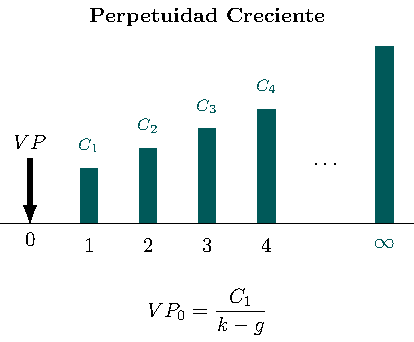
\includegraphics[width=5cm]{\rutaImagenes/capitalizacion_directa}\\
	
	\begin{minipage}{5cm}
	Where
	\begin{itemize}
	

	
		\item $C_1$: Cash Flow
		\item $k$: Capitalization rate
		\item $g$: Growth rate
	\end{itemize}
	\end{minipage}
\end{figure}
\end{center}



\textcolor{principal}{Capitalization using a growing perpetuity} refers to the case where the value of an income stream shows a noticeable and consistent upward trend over successive annual periods. In terms of investments, this often translates into a situation where the anticipated annual return from the investment is consistently met or even exceeded from one year to the next. The concept also implies that this cash flow will continue into the foreseeable future if the investor chooses to retain the asset over many years.\\

Evaluating the potential for a growing perpetuity is often very important for investors who wish to acquire a given investment with the aim of holding that investment over several years. Part of the process of accurately assessing the presence of a growing perpetuity year over year involves considering changes in the overall state of the economy. This means that it may be necessary to adjust figures for a given year to offset the effect of inflation.\\[10pt]
